%%%%%%%%%%%%%%%%
\documentclass[aspectratio=169,xcolor={dvipsnames,table}]{beamer}
\usepackage[no-math,deluxe,haranoaji]{luatexja-preset}
\renewcommand{\kanjifamilydefault}{\gtdefault}
\renewcommand{\emph}[1]{{\upshape\bfseries #1}}
\usetheme{metropolis}
\metroset{block=fill}
%%%%%%%%%%%%%%%%%%%%%%%%%%%
\usepackage{figchild}
%%%%%%%%%%%%%%%%%%%%%%%%%%%
\usepackage{tikzducks}
\usepackage{worldflags}
%%%%%%%%%%%%%%%%%%%%%%%%%%
%% TEXT
%%%%%%%%%%%%%%%%%%%%%%%%%%%%
\begin{document}
%%%%%%%%%%%%%%%%%%%%%%%%%%%%
\begin{frame}[plain]{oyoyo}

\begin{center}
\fcTrain[draw=gray, line width = 2, scale=2]
\end{center}
\end{frame}
%%%%%%%%%%%%%%%%%%%%%
\begin{frame}[plain]{oyoyo}

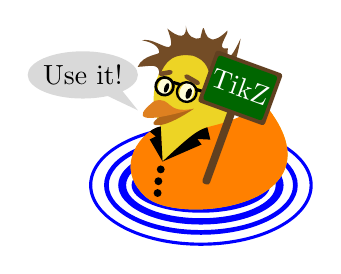
\begin{tikzpicture}
  \duck[crazyhair=brown!60!black, glasses, eyebrow,
    signpost=TikZ, speech=Use it!, laughing,
    jacket=orange, lapel, buttons, water]
\end{tikzpicture}
%
%\worldflag[width=2cm,framewidth=0.3mm,framecolor=black]{BR}
\end{frame}
%%%%%%%%%%%%%%%%%%%%%%%%%%%%%%%%%%%%
\end{document}
%\documentclass[tikz,border=10pt]{standalone}
\documentclass[aspectratio=169,xcolor={dvipsnames,table}]{beamer}
\usepackage[no-math,deluxe,haranoaji]{luatexja-preset}
\renewcommand{\kanjifamilydefault}{\gtdefault}
\renewcommand{\emph}[1]{{\upshape\bfseries #1}}
\usetheme{metropolis}
\metroset{block=fill}
%\usepackage{figchild}
\usepackage{worldflags}
\begin{document}
\worldflag[width=2cm,framewidth=0.3mm,framecolor=black]{BR}
\end{document}
